Le système est composé des éléments suivants
% , comme illustré dans la figure \textbf{\ref{fig:system_architecture}} 
:

\begin{itemize}
    \item \textbf{Serveur Local / Cloud} :
    \begin{itemize}
        \item \textbf{Backend} : Traitement des données et gestion des alertes.
        \item \textbf{Base de Données} : Stockage des données des patients et des alertes.
        \item \textbf{Service de Notifications} : Envoi d’alertes (e-mails, notifications push).
    \end{itemize}
    \item \textbf{Appareils Médicaux} :
    \begin{itemize}
        \item \textbf{Moniteur Mindray} : Envoie les données via API HL7.
        \item \textbf{Caméra OCR} : Capture et extrait les valeurs vitales.
    \end{itemize}
    \item \textbf{Applications Mobiles \& Web} :
    \begin{itemize}
        \item \textbf{Application Web / Mobile} : Consultation des données via REST API.
    \end{itemize}
\end{itemize}

% \begin{figure}[H]
%     \centering
%     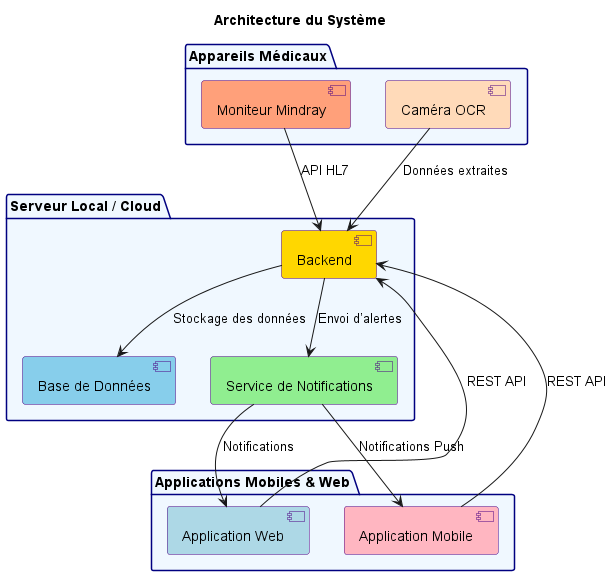
\includegraphics[width=0.8\textwidth]{chapter2/sections/diagrams/system_architecture.png}
%     \caption{Architecture du Système}
%     \label{fig:system_architecture}
% \end{figure}